\section{Introduction and Design}
This report presents the implementation of a relative intensity vision sensor pixel, intended for use in 
an asynchronous line sensor. 
\begin{figure}
    \center
    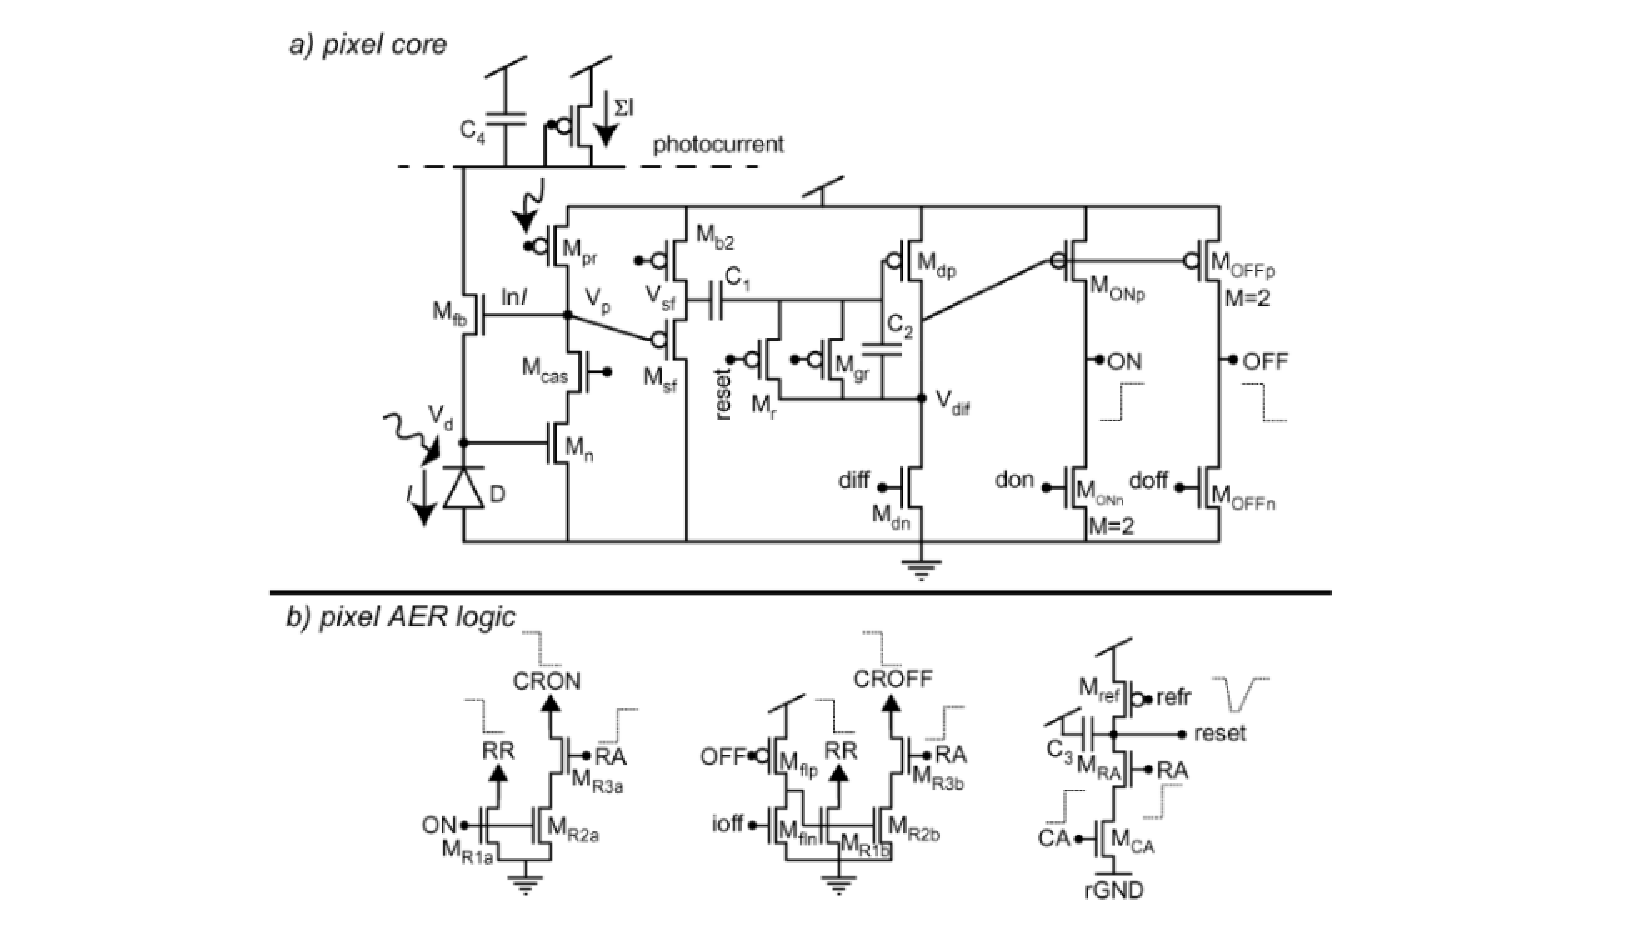
\includegraphics[trim={4.5cm 0 4.5cm 0},clip,width=\textwidth]{pixel-design.eps}
    \caption{(a) schematic of the pixel design and (b) digital circuits for AER logic interfacing, of these only the 
    third from the left is used as the others are unnecessary for a one-dimensional sensor. Transistor sizes (W/L) in
    (\(\mu\)m,\(\mu\)m) and capacitor values are as follows: \(M_{fb}\) 2/2, \(M_{pr}\) 6/2, \(M_{cas}\) 4/4, \(M_n\) 4/4,
    \(M_{b2}\) 4/4, \(M_{sf}\) 4/4, \(M_r\) 0.540/0.180, \(M_{gr}\) 0.540/0.180, \(M_{dp}\) 6/2, \(M_{dn}\) 4/4,
    \(M_{ONp}\) 6/2, \(M_{ONn}\) 4/4, \(M_{OFFp}\) 6/2, \(M_{OFFn}\) 4/4, \(M_{ref}\) 6/2, \(M_{RA}\) 4/4, \(M_{CA}\) 4/4,
    C1 2.84 pF, C2 50 fF and C3 30 fF. \(\Sigma I\) and C4 are unused. Reproduced from~\cite{Lichtsteiner2008}}
    \label{fig:pixel-design}
\end{figure}
We will use the pixel design by Lichtsteiner et al.~\cite{Lichtsteiner2008}, which is reproduced in Fig~\ref{fig:pixel-design}.
The modifications to the referenced design will be evaluated by the following figure of merit (FOM)
\begin{equation}
    \text{FOM} = \frac{\text{bandwidth}}{P_{\text{avg}}\cdot \text{mismatch\%}\cdot L}
    \label{eq:FOM}
\end{equation}
Where \(P_{\text{avg}}\) is the average power consumption for our fixed evaluation input signal, mismatch is the 
\(3\sigma\) change in relative light intensity sensitivity due to mismatch, and \(L\) is the length of the pixel in feature units (180 nm).
Additionally, a factor 3.3 change in contrast must produce a mean of 12 events, and the width of the pixel is
limited to 8.6 \(\mu\)m. This is the minimum possible pixel pitch because of the mimcap layer spacing rules in the 
process we use.
Clearly it is impossible to obtain zero power consumption or length for a functioning pixel.
Therefore, we chose to attempt a design which is completely invariant to mismatch within the limits given by
the AMS180 process in order to obtain a maximal FOM. 

The uniformity of response in the number of events generated from a fixed stimulus is higher when the on and off
thresholds are high. However, the total number of events will drop with increasing threshold. 
Because of this, we must employ a very large gain in the differencing circuit to maintain a mean of 12 events
for a change in contrast by a factor of 3.3 if we wish to have high thresholds.
Therefore, we choose a gain in the differencing circuit of ~60. With such a gain, the sizes of the 
transistors become near irrelevant because of the large area under the capacitors, which they can occupy without
affecting the length of the pixel.


